%%%%%%%%%%%%%%%%%%%%%%%%%%%%%%%%%%%%%%%%%%%%%%%%%%%%%%%%%%%%
% 1.4 GROUP THEORY
% The Composition of Advanced Mathematics
%%%%%%%%%%%%%%%%%%%%%%%%%%%%%%%%%%%%%%%%%%%%%%%%%%%%%%%%%%%%

\section{Group Theory}
\label{sec:group-theory}

\prerequisite{
Elementary set theory from \cref{sec:elementary-set-theory}, relations from
\cref{sec:relations}, functions from \cref{sec:functions}, methods of proof
from \cref{sec:methods-of-proof}, and the structural language of abstract
algebra from \cref{sec:abstract-algebra}.
}

\learningobjectives{
By the end of this section, the reader should be able to:
\begin{itemize}
    \item verify whether a set and operation form a group;
    \item distinguish abelian and nonabelian groups;
    \item use identities, inverses, cancellation, and exponent laws;
    \item identify and prove that subsets are subgroups;
    \item work with cyclic groups and generators;
    \item determine the order of elements and finite groups;
    \item work with permutation groups and cycle notation;
    \item interpret symmetry groups geometrically;
    \item compute left and right cosets;
    \item apply Lagrange's theorem;
    \item recognize normal subgroups;
    \item construct and interpret quotient groups;
    \item work with group homomorphisms, kernels, and images;
    \item apply the First Isomorphism Theorem;
    \item understand direct products of groups;
    \item recognize the role of group actions and orbits;
    \item use structural arguments rather than relying only on computation.
\end{itemize}
}

%%%%%%%%%%%%%%%%%%%%%%%%%%%%%%%%%%%%%%%%%%%%%%%%%%%%%%%%%%%%
\subsection{The Central Idea of Group Theory}
\label{subsec:central-idea-group-theory}
%%%%%%%%%%%%%%%%%%%%%%%%%%%%%%%%%%%%%%%%%%%%%%%%%%%%%%%%%%%%

A group is one of the fundamental structures of modern mathematics.

Groups arise whenever mathematical objects can be combined in a reversible
and associative way.

Important examples include:

\begin{itemize}
    \item integers under addition;
    \item nonzero real numbers under multiplication;
    \item invertible matrices under matrix multiplication;
    \item permutations under composition;
    \item rotations and reflections of geometric objects;
    \item transformations preserving mathematical structures.
\end{itemize}

\begin{conceptbox}
Group theory studies symmetry, reversible transformations, and algebraic
systems governed by one associative operation with an identity and inverses.
\end{conceptbox}

The objects inside a group may be numbers, matrices, functions,
transformations, permutations, or something entirely different.

What matters is how the elements interact.

%%%%%%%%%%%%%%%%%%%%%%%%%%%%%%%%%%%%%%%%%%%%%%%%%%%%%%%%%%%%
\subsection{Definition of a Group}
\label{subsec:definition-group}
%%%%%%%%%%%%%%%%%%%%%%%%%%%%%%%%%%%%%%%%%%%%%%%%%%%%%%%%%%%%

\begin{definitionbox}{Group}
A \emph{group} is a set \(G\) equipped with a binary operation
\[ *:G\times G\to G \]
satisfying the following axioms for all \(a,b,c\in G\):

\begin{enumerate}
    \item \textbf{Closure:}
    \[ a*b\in G. \]

    \item \textbf{Associativity:}
    \[ (a*b)*c=a*(b*c). \]

    \item \textbf{Identity:}
    there exists \(e\in G\) such that
    \[ e*a=a*e=a. \]

    \item \textbf{Inverses:}
    for every \(a\in G\), there exists \(a^{-1}\in G\) such that
    \[ a*a^{-1}=a^{-1}*a=e. \]
\end{enumerate}
\end{definitionbox}

A group is commonly written

\[ (G,*). \]

If the operation is understood, one often writes simply \(G\).

%%%%%%%%%%%%%%%%%%%%%%%%%%%%%%%%%%%%%%%%%%%%%%%%%%%%%%%%%%%%
\subsection{Multiplicative and Additive Notation}
\label{subsec:additive-multiplicative-group-notation}
%%%%%%%%%%%%%%%%%%%%%%%%%%%%%%%%%%%%%%%%%%%%%%%%%%%%%%%%%%%%

Groups are commonly written in one of two notational styles.

In \emph{multiplicative notation},

\[ ab \]

means the group operation applied to \(a\) and \(b\).

The identity is written

\[ e, \]

and the inverse is

\[ a^{-1}. \]

In \emph{additive notation},

\[ a+b \]

denotes the operation, the identity is \(0\), and the inverse of \(a\) is
\(-a\).

Additive notation is especially common for abelian groups.

%%%%%%%%%%%%%%%%%%%%%%%%%%%%%%%%%%%%%%%%%%%%%%%%%%%%%%%%%%%%
\subsection{Abelian Groups}
\label{subsec:abelian-groups}
%%%%%%%%%%%%%%%%%%%%%%%%%%%%%%%%%%%%%%%%%%%%%%%%%%%%%%%%%%%%

\begin{definitionbox}{Abelian Group}
A group \(G\) is \emph{abelian} if
\[ ab=ba \]
for every \(a,b\in G\).
\end{definitionbox}

The term \emph{abelian} honors the mathematician Niels Henrik Abel.

Examples include

\[ (\Z,+),\qquad (\Q,+),\qquad (\R,+). \]

Not every group is abelian.

Matrix groups and symmetry groups frequently provide counterexamples.

%%%%%%%%%%%%%%%%%%%%%%%%%%%%%%%%%%%%%%%%%%%%%%%%%%%%%%%%%%%%
\subsection{First Examples of Groups}
\label{subsec:first-group-examples}
%%%%%%%%%%%%%%%%%%%%%%%%%%%%%%%%%%%%%%%%%%%%%%%%%%%%%%%%%%%%

The integers under addition form a group:

\[ (\Z,+). \]

The identity is \(0\), and the inverse of \(a\) is \(-a\).

The nonzero real numbers under multiplication form a group:

\[ (\R\setminus\{0\},\cdot). \]

The identity is \(1\), and the inverse of \(a\) is \(1/a\).

The natural numbers under addition do not form a group because additive
inverses are generally missing.

%%%%%%%%%%%%%%%%%%%%%%%%%%%%%%%%%%%%%%%%%%%%%%%%%%%%%%%%%%%%
\subsection{Groups of Matrices}
\label{subsec:matrix-groups}
%%%%%%%%%%%%%%%%%%%%%%%%%%%%%%%%%%%%%%%%%%%%%%%%%%%%%%%%%%%%

Invertible matrices provide an important family of nontrivial groups.

\begin{definitionbox}{General Linear Group}
The \emph{general linear group} of degree \(n\) over a field \(F\) is
\[ GL_n(F)=\{A\in M_n(F):\det(A)\neq0\}, \]
with matrix multiplication as the group operation.
\end{definitionbox}

The notation

\[ GL_n(F) \]

is read ``general linear group of degree \(n\) over \(F\).''

The identity element is the identity matrix

\[ I_n, \]

and the inverse of \(A\) is its matrix inverse \(A^{-1}\).

Matrix multiplication is generally noncommutative, so

\[ AB\neq BA \]

may occur.

Thus \(GL_n(F)\) is generally nonabelian.

%%%%%%%%%%%%%%%%%%%%%%%%%%%%%%%%%%%%%%%%%%%%%%%%%%%%%%%%%%%%
\subsection{Elementary Consequences of the Group Axioms}
\label{subsec:group-axiom-consequences}
%%%%%%%%%%%%%%%%%%%%%%%%%%%%%%%%%%%%%%%%%%%%%%%%%%%%%%%%%%%%

The four group axioms imply many additional properties.

These properties do not need to be assumed separately.

%%%%%%%%%%%%%%%%%%%%%%%%%%%%%%%%%%%%%%%%%%%%%%%%%%%%%%%%%%%%
\subsection{Uniqueness of the Identity}
\label{subsec:group-identity-unique}
%%%%%%%%%%%%%%%%%%%%%%%%%%%%%%%%%%%%%%%%%%%%%%%%%%%%%%%%%%%%

\begin{theorem}
A group has exactly one identity element.
\end{theorem}

\begin{proof}
Suppose \(e\) and \(f\) are both identity elements.

Since \(e\) is an identity,

\[ ef=f. \]

Since \(f\) is an identity,

\[ ef=e. \]

Therefore,

\[ e=f. \]
\end{proof}

%%%%%%%%%%%%%%%%%%%%%%%%%%%%%%%%%%%%%%%%%%%%%%%%%%%%%%%%%%%%
\subsection{Uniqueness of Inverses}
\label{subsec:group-inverses-unique}
%%%%%%%%%%%%%%%%%%%%%%%%%%%%%%%%%%%%%%%%%%%%%%%%%%%%%%%%%%%%

\begin{theorem}
Every element of a group has exactly one inverse.
\end{theorem}

\begin{proof}
Suppose \(b\) and \(c\) are both inverses of \(a\).

Then

\[ ab=e,\qquad ca=e. \]

Therefore,

\[
\begin{aligned}
b
&=be\\
&=b(ac)\\
&=(ba)c\\
&=ec\\
&=c.
\end{aligned}
\]

Hence the inverse of \(a\) is unique.
\end{proof}

%%%%%%%%%%%%%%%%%%%%%%%%%%%%%%%%%%%%%%%%%%%%%%%%%%%%%%%%%%%%
\subsection{Cancellation Laws}
\label{subsec:group-cancellation-laws}
%%%%%%%%%%%%%%%%%%%%%%%%%%%%%%%%%%%%%%%%%%%%%%%%%%%%%%%%%%%%

\begin{theorem}[Cancellation Laws]
For \(a,b,c\in G\),

\[ ab=ac\Longrightarrow b=c \]

and

\[ ba=ca\Longrightarrow b=c. \]
\end{theorem}

\begin{proof}
Suppose

\[ ab=ac. \]

Multiply both sides on the left by \(a^{-1}\):

\[ a^{-1}(ab)=a^{-1}(ac). \]

Associativity gives

\[ (a^{-1}a)b=(a^{-1}a)c. \]

Therefore,

\[ eb=ec, \]

so

\[ b=c. \]

The right cancellation law follows similarly.
\end{proof}

%%%%%%%%%%%%%%%%%%%%%%%%%%%%%%%%%%%%%%%%%%%%%%%%%%%%%%%%%%%%
\subsection{Solving Group Equations}
\label{subsec:solving-group-equations}
%%%%%%%%%%%%%%%%%%%%%%%%%%%%%%%%%%%%%%%%%%%%%%%%%%%%%%%%%%%%

Consider

\[ ax=b. \]

Multiply on the left by \(a^{-1}\):

\[ a^{-1}(ax)=a^{-1}b. \]

Therefore,

\[ x=a^{-1}b. \]

For

\[ xa=b, \]

multiply on the right:

\[ x=ba^{-1}. \]

\begin{warningbox}
In a nonabelian group, order matters.

In general,
\[ a^{-1}b\neq ba^{-1}. \]

One cannot move group elements across an equation as though ordinary
commutative arithmetic were being used.
\end{warningbox}

%%%%%%%%%%%%%%%%%%%%%%%%%%%%%%%%%%%%%%%%%%%%%%%%%%%%%%%%%%%%
\subsection{Inverse of a Product}
\label{subsec:inverse-product-group}
%%%%%%%%%%%%%%%%%%%%%%%%%%%%%%%%%%%%%%%%%%%%%%%%%%%%%%%%%%%%

\begin{theorem}
For \(a,b\in G\),
\[ (ab)^{-1}=b^{-1}a^{-1}. \]
\end{theorem}

\begin{proof}
Compute

\[ (ab)(b^{-1}a^{-1})=a(bb^{-1})a^{-1}=aea^{-1}=aa^{-1}=e. \]

Similarly,

\[ (b^{-1}a^{-1})(ab)=b^{-1}(a^{-1}a)b=b^{-1}eb=b^{-1}b=e. \]

Therefore,

\[ (ab)^{-1}=b^{-1}a^{-1}. \]
\end{proof}

The order reverses.

For a longer product,

\[ (a_1a_2\cdots a_n)^{-1}=a_n^{-1}\cdots a_2^{-1}a_1^{-1}. \]

%%%%%%%%%%%%%%%%%%%%%%%%%%%%%%%%%%%%%%%%%%%%%%%%%%%%%%%%%%%%
\subsection{Powers of Group Elements}
\label{subsec:group-powers}
%%%%%%%%%%%%%%%%%%%%%%%%%%%%%%%%%%%%%%%%%%%%%%%%%%%%%%%%%%%%

For \(a\in G\),

\[ a^1=a,\qquad a^2=aa,\qquad a^3=aaa. \]

Define

\[ a^0=e \]

and, for positive \(n\),

\[ a^{-n}=(a^{-1})^n. \]

The familiar exponent laws remain valid for powers of a single group element:

\[ a^ma^n=a^{m+n},\qquad (a^m)^n=a^{mn}. \]

However, in a nonabelian group,

\[ (ab)^n=a^nb^n \]

is generally false.

%%%%%%%%%%%%%%%%%%%%%%%%%%%%%%%%%%%%%%%%%%%%%%%%%%%%%%%%%%%%
\subsection{Order of a Group}
\label{subsec:order-group}
%%%%%%%%%%%%%%%%%%%%%%%%%%%%%%%%%%%%%%%%%%%%%%%%%%%%%%%%%%%%

\begin{definitionbox}{Order of a Group}
The \emph{order} of a finite group \(G\), written
\[ |G|, \]
is the number of elements in \(G\).
\end{definitionbox}

The notation \(|G|\) is read ``the order of \(G\)'' in group theory.

For example, if

\[ G=\{e,a,b,c\}, \]

then

\[ |G|=4. \]

For infinite groups, one may simply say the group has infinite order.

%%%%%%%%%%%%%%%%%%%%%%%%%%%%%%%%%%%%%%%%%%%%%%%%%%%%%%%%%%%%
\subsection{Order of an Element}
\label{subsec:order-element}
%%%%%%%%%%%%%%%%%%%%%%%%%%%%%%%%%%%%%%%%%%%%%%%%%%%%%%%%%%%%

\begin{definitionbox}{Order of an Element}
The \emph{order} of an element \(a\in G\), written
\[ |a|, \]
is the smallest positive integer \(n\) such that
\[ a^n=e. \]

If no such positive integer exists, \(a\) has infinite order.
\end{definitionbox}

The meaning of vertical bars here is determined by context.

For example, in the additive group \(\Z\), the element \(1\) has infinite
order.

%%%%%%%%%%%%%%%%%%%%%%%%%%%%%%%%%%%%%%%%%%%%%%%%%%%%%%%%%%%%
\subsection{Cyclic Groups}
\label{subsec:cyclic-groups}
%%%%%%%%%%%%%%%%%%%%%%%%%%%%%%%%%%%%%%%%%%%%%%%%%%%%%%%%%%%%

\begin{definitionbox}{Cyclic Group}
A group \(G\) is \emph{cyclic} if there exists \(a\in G\) such that
\[ G=\langle a\rangle. \]

The element \(a\) is called a \emph{generator} of \(G\).
\end{definitionbox}

In multiplicative notation,

\[ \langle a\rangle=\{a^n:n\in\Z\}. \]

In additive notation,

\[ \langle a\rangle=\{na:n\in\Z\}. \]

%%%%%%%%%%%%%%%%%%%%%%%%%%%%%%%%%%%%%%%%%%%%%%%%%%%%%%%%%%%%
\subsection{Visualizing a Finite Cyclic Group}
\label{subsec:visual-cyclic-group}
%%%%%%%%%%%%%%%%%%%%%%%%%%%%%%%%%%%%%%%%%%%%%%%%%%%%%%%%%%%%

Consider the cyclic group of order \(6\).

\begin{center}
\begin{tikzpicture}[scale=1.05,>=stealth]
\foreach \k in {0,...,5}{
    \node[circle,draw,minimum size=8mm] (n\k) at ({90-60*\k}:2.1) {\(\k\)};
}
\foreach \k [evaluate=\k as \next using int(mod(\k+1,6))] in {0,...,5}{
    \draw[->,thick] (n\k) to[bend left=14] (n\next);
}
\node at (4.2,0.4) {add \(1\)};
\node at (4.2,-0.2) {modulo \(6\)};
\end{tikzpicture}
\end{center}

Starting at \(0\) and repeatedly adding \(1\) reaches every element.

Thus \(1\) generates the group.

%%%%%%%%%%%%%%%%%%%%%%%%%%%%%%%%%%%%%%%%%%%%%%%%%%%%%%%%%%%%
\subsection{Every Cyclic Group Is Abelian}
\label{subsec:cyclic-groups-abelian}
%%%%%%%%%%%%%%%%%%%%%%%%%%%%%%%%%%%%%%%%%%%%%%%%%%%%%%%%%%%%

\begin{theorem}
Every cyclic group is abelian.
\end{theorem}

\begin{proof}
Suppose

\[ G=\langle a\rangle. \]

Then every \(x,y\in G\) can be written

\[ x=a^m,\qquad y=a^n \]

for integers \(m,n\).

Therefore,

\[ xy=a^ma^n=a^{m+n}=a^{n+m}=a^na^m=yx. \]

Hence \(G\) is abelian.
\end{proof}

%%%%%%%%%%%%%%%%%%%%%%%%%%%%%%%%%%%%%%%%%%%%%%%%%%%%%%%%%%%%
\subsection{Subgroups}
\label{subsec:subgroups}
%%%%%%%%%%%%%%%%%%%%%%%%%%%%%%%%%%%%%%%%%%%%%%%%%%%%%%%%%%%%

\begin{definitionbox}{Subgroup}
A subset \(H\subseteq G\) is a \emph{subgroup} of \(G\) if \(H\) itself forms
a group under the operation inherited from \(G\).
\end{definitionbox}

The notation

\[ H\leq G \]

is read ``\(H\) is a subgroup of \(G\).''

Every group has at least two natural subgroup candidates:

\[ \{e\}\qquad\text{and}\qquad G. \]

The subgroup \(\{e\}\) is called the \emph{trivial subgroup}.

%%%%%%%%%%%%%%%%%%%%%%%%%%%%%%%%%%%%%%%%%%%%%%%%%%%%%%%%%%%%
\subsection{Visualizing a Subgroup}
\label{subsec:visual-subgroup}
%%%%%%%%%%%%%%%%%%%%%%%%%%%%%%%%%%%%%%%%%%%%%%%%%%%%%%%%%%%%

\begin{center}
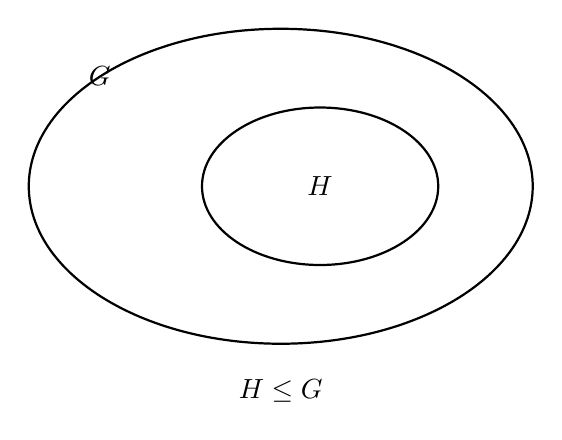
\begin{tikzpicture}
\draw[thick] (0,0) ellipse (3.2 and 2);
\draw[thick] (0.5,0) ellipse (1.5 and 1);
\node at (-2.3,1.4) {\(G\)};
\node at (0.5,0) {\(H\)};
\node at (0,-2.6) {\(H\leq G\)};
\end{tikzpicture}
\end{center}

A subgroup is not merely a subset. It must retain the group structure.

%%%%%%%%%%%%%%%%%%%%%%%%%%%%%%%%%%%%%%%%%%%%%%%%%%%%%%%%%%%%
\subsection{The Subgroup Test}
\label{subsec:subgroup-test}
%%%%%%%%%%%%%%%%%%%%%%%%%%%%%%%%%%%%%%%%%%%%%%%%%%%%%%%%%%%%

Checking all four group axioms every time is unnecessary.

\begin{theorem}[Subgroup Test]
Let \(H\) be a nonempty subset of a group \(G\). Then \(H\leq G\) if
\[ a,b\in H\Longrightarrow ab^{-1}\in H. \]
\end{theorem}

This single condition encodes closure and inverses, while associativity is
inherited from \(G\).

%%%%%%%%%%%%%%%%%%%%%%%%%%%%%%%%%%%%%%%%%%%%%%%%%%%%%%%%%%%%
\subsection{Worked Example: Proving a Subgroup}
\label{subsec:worked-subgroup}
%%%%%%%%%%%%%%%%%%%%%%%%%%%%%%%%%%%%%%%%%%%%%%%%%%%%%%%%%%%%

\begin{workedexamplebox}{The Even Integers as a Subgroup}

Show that

\[ 2\Z=\{2k:k\in\Z\} \]

is a subgroup of \((\Z,+)\).

\begin{tabularx}{\textwidth}{@{}>{\raggedright\arraybackslash}p{0.42\textwidth}X@{}}
Take arbitrary elements. & \(a=2m,\quad b=2n\)\\
Use the additive subgroup test. & \(a-b=2m-2n\)\\
Factor. & \(a-b=2(m-n)\)\\
Use integer closure. & \(m-n\in\Z\)
\end{tabularx}

Thus \(a-b\in2\Z\).

\begin{answerbox}
\[ 2\Z\leq\Z. \]
\end{answerbox}
\end{workedexamplebox}

%%%%%%%%%%%%%%%%%%%%%%%%%%%%%%%%%%%%%%%%%%%%%%%%%%%%%%%%%%%%
\subsection{Intersection of Subgroups}
\label{subsec:intersection-subgroups}
%%%%%%%%%%%%%%%%%%%%%%%%%%%%%%%%%%%%%%%%%%%%%%%%%%%%%%%%%%%%

\begin{theorem}
If \(H\leq G\) and \(K\leq G\), then
\[ H\cap K\leq G. \]
\end{theorem}

More generally, the intersection of any nonempty family of subgroups of \(G\)
is again a subgroup.

Unions behave differently.

In general,

\[ H\cup K \]

need not be a subgroup.

%%%%%%%%%%%%%%%%%%%%%%%%%%%%%%%%%%%%%%%%%%%%%%%%%%%%%%%%%%%%
\subsection{Generated Subgroups}
\label{subsec:generated-subgroups}
%%%%%%%%%%%%%%%%%%%%%%%%%%%%%%%%%%%%%%%%%%%%%%%%%%%%%%%%%%%%

If \(S\subseteq G\), the subgroup generated by \(S\) is written

\[ \langle S\rangle. \]

It is the smallest subgroup of \(G\) containing \(S\).

Equivalently,

\[ \langle S\rangle=\bigcap_{\substack{H\leq G\\S\subseteq H}}H. \]

This expression says to intersect every subgroup containing \(S\).

%%%%%%%%%%%%%%%%%%%%%%%%%%%%%%%%%%%%%%%%%%%%%%%%%%%%%%%%%%%%
\subsection{Permutation Groups}
\label{subsec:permutation-groups}
%%%%%%%%%%%%%%%%%%%%%%%%%%%%%%%%%%%%%%%%%%%%%%%%%%%%%%%%%%%%

A \emph{permutation} is a bijection from a set to itself.

For the set

\[ \{1,2,\ldots,n\}, \]

all permutations form the \emph{symmetric group}.

\begin{definitionbox}{Symmetric Group}
The symmetric group on \(n\) symbols is denoted
\[ S_n. \]

Its operation is composition of permutations.
\end{definitionbox}

The notation \(S_n\) is read ``S sub \(n\)'' or ``the symmetric group on
\(n\) symbols.''

There are

\[ n! \]

permutations of \(n\) objects, so

\[ |S_n|=n!. \]

%%%%%%%%%%%%%%%%%%%%%%%%%%%%%%%%%%%%%%%%%%%%%%%%%%%%%%%%%%%%
\subsection{Two-Line Permutation Notation}
\label{subsec:two-line-permutations}
%%%%%%%%%%%%%%%%%%%%%%%%%%%%%%%%%%%%%%%%%%%%%%%%%%%%%%%%%%%%

A permutation may be written

\[
\sigma=
\begin{pmatrix}
1&2&3&4\\
2&4&1&3
\end{pmatrix}.
\]

The symbol

\[ \sigma \]

is lowercase Greek \emph{sigma}, pronounced ``SIG-muh.''

This permutation sends

\[ 1\mapsto2,\qquad2\mapsto4,\qquad3\mapsto1,\qquad4\mapsto3. \]

%%%%%%%%%%%%%%%%%%%%%%%%%%%%%%%%%%%%%%%%%%%%%%%%%%%%%%%%%%%%
\subsection{Cycle Notation}
\label{subsec:cycle-notation}
%%%%%%%%%%%%%%%%%%%%%%%%%%%%%%%%%%%%%%%%%%%%%%%%%%%%%%%%%%%%

The same permutation can often be represented more compactly using cycles.

For example,

\[ (1\,2\,4\,3) \]

means

\[ 1\mapsto2,\quad2\mapsto4,\quad4\mapsto3,\quad3\mapsto1. \]

The expression is read

\begin{center}
``the cycle one, two, four, three.''
\end{center}

A cycle of length \(k\) is called a \(k\)-cycle.

%%%%%%%%%%%%%%%%%%%%%%%%%%%%%%%%%%%%%%%%%%%%%%%%%%%%%%%%%%%%
\subsection{Visualizing a Cycle}
\label{subsec:visual-cycle}
%%%%%%%%%%%%%%%%%%%%%%%%%%%%%%%%%%%%%%%%%%%%%%%%%%%%%%%%%%%%

\begin{center}
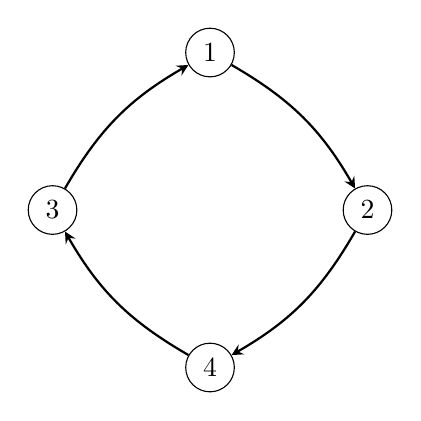
\begin{tikzpicture}[>=stealth]
\node[circle,draw] (1) at (0,2) {\(1\)};
\node[circle,draw] (2) at (2,0) {\(2\)};
\node[circle,draw] (4) at (0,-2) {\(4\)};
\node[circle,draw] (3) at (-2,0) {\(3\)};

\draw[->,thick] (1) to[bend left=15] (2);
\draw[->,thick] (2) to[bend left=15] (4);
\draw[->,thick] (4) to[bend left=15] (3);
\draw[->,thick] (3) to[bend left=15] (1);
\end{tikzpicture}
\end{center}

The diagram directly represents

\[ (1\,2\,4\,3). \]

%%%%%%%%%%%%%%%%%%%%%%%%%%%%%%%%%%%%%%%%%%%%%%%%%%%%%%%%%%%%
\subsection{Disjoint Cycles}
\label{subsec:disjoint-cycles}
%%%%%%%%%%%%%%%%%%%%%%%%%%%%%%%%%%%%%%%%%%%%%%%%%%%%%%%%%%%%

Cycles are \emph{disjoint} if they move different elements.

For example,

\[ (1\,3\,5)(2\,4) \]

contains two disjoint cycles.

Disjoint cycles commute.

Thus,

\[ (1\,3\,5)(2\,4)=(2\,4)(1\,3\,5). \]

Every permutation can be written as a product of disjoint cycles.

%%%%%%%%%%%%%%%%%%%%%%%%%%%%%%%%%%%%%%%%%%%%%%%%%%%%%%%%%%%%
\subsection{Transpositions}
\label{subsec:transpositions}
%%%%%%%%%%%%%%%%%%%%%%%%%%%%%%%%%%%%%%%%%%%%%%%%%%%%%%%%%%%%

A cycle that exchanges exactly two elements is called a
\emph{transposition}.

For example,

\[ (1\,4) \]

exchanges \(1\) and \(4\).

Every permutation can be written as a product of transpositions.

This fact leads to the distinction between even and odd permutations.

%%%%%%%%%%%%%%%%%%%%%%%%%%%%%%%%%%%%%%%%%%%%%%%%%%%%%%%%%%%%
\subsection{Even and Odd Permutations}
\label{subsec:even-odd-permutations}
%%%%%%%%%%%%%%%%%%%%%%%%%%%%%%%%%%%%%%%%%%%%%%%%%%%%%%%%%%%%

A permutation is \emph{even} if it can be expressed as a product of an even
number of transpositions.

It is \emph{odd} if it requires an odd number.

The parity of a permutation is well defined: a permutation cannot be both
even and odd.

%%%%%%%%%%%%%%%%%%%%%%%%%%%%%%%%%%%%%%%%%%%%%%%%%%%%%%%%%%%%
\subsection{Alternating Groups}
\label{subsec:alternating-groups}
%%%%%%%%%%%%%%%%%%%%%%%%%%%%%%%%%%%%%%%%%%%%%%%%%%%%%%%%%%%%

\begin{definitionbox}{Alternating Group}
The \emph{alternating group} \(A_n\) consists of all even permutations in
\(S_n\).
\end{definitionbox}

For \(n\geq2\),

\[ |A_n|=\frac{n!}{2}. \]

Alternating groups later become especially important in Galois theory and the
study of polynomial equations.

%%%%%%%%%%%%%%%%%%%%%%%%%%%%%%%%%%%%%%%%%%%%%%%%%%%%%%%%%%%%
\subsection{Symmetry Groups}
\label{subsec:symmetry-groups}
%%%%%%%%%%%%%%%%%%%%%%%%%%%%%%%%%%%%%%%%%%%%%%%%%%%%%%%%%%%%

A symmetry of a geometric object is a transformation that preserves its
overall shape.

For a square, symmetries include rotations and reflections.

\begin{center}
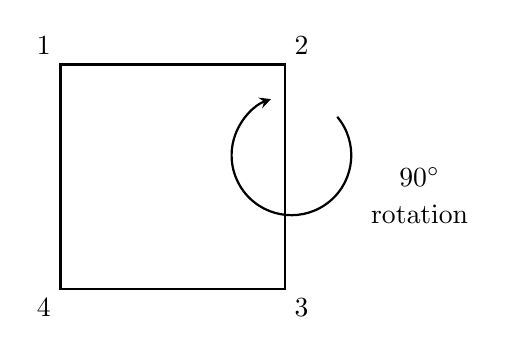
\begin{tikzpicture}[scale=0.95,>=stealth]
\coordinate (A) at (-1.5,1.5);
\coordinate (B) at (1.5,1.5);
\coordinate (C) at (1.5,-1.5);
\coordinate (D) at (-1.5,-1.5);

\draw[thick] (A)--(B)--(C)--(D)--cycle;

\node[above left] at (A) {\(1\)};
\node[above right] at (B) {\(2\)};
\node[below right] at (C) {\(3\)};
\node[below left] at (D) {\(4\)};

\draw[->,thick] (2.2,0.8) arc[start angle=40,end angle=-250,radius=0.8];
\node at (3.3,0) {\(90^\circ\)};
\node at (3.3,-0.5) {rotation};
\end{tikzpicture}
\end{center}

Combining two symmetries gives another symmetry, and every symmetry can be
undone.

Thus the symmetries form a group.

%%%%%%%%%%%%%%%%%%%%%%%%%%%%%%%%%%%%%%%%%%%%%%%%%%%%%%%%%%%%
\subsection{Dihedral Groups}
\label{subsec:dihedral-groups}
%%%%%%%%%%%%%%%%%%%%%%%%%%%%%%%%%%%%%%%%%%%%%%%%%%%%%%%%%%%%

\begin{definitionbox}{Dihedral Group}
The \emph{dihedral group} \(D_n\) is the group of rotational and reflectional
symmetries of a regular \(n\)-gon.
\end{definitionbox}

Under the convention used here,

\[ |D_n|=2n. \]

There are \(n\) rotations and \(n\) reflections.

\begin{notebox}
Some texts use \(D_{2n}\) for the group of order \(2n\). Always check the
author's convention.
\end{notebox}

%%%%%%%%%%%%%%%%%%%%%%%%%%%%%%%%%%%%%%%%%%%%%%%%%%%%%%%%%%%%
\subsection{The Symmetry Group of a Square}
\label{subsec:square-symmetry-group}
%%%%%%%%%%%%%%%%%%%%%%%%%%%%%%%%%%%%%%%%%%%%%%%%%%%%%%%%%%%%

The square has eight symmetries.

Four are rotations:

\[ e,\qquad r,\qquad r^2,\qquad r^3. \]

Four are reflections.

Thus

\[ |D_4|=8. \]

The rotation \(r\) satisfies

\[ r^4=e. \]

If \(s\) is an appropriate reflection, then

\[ s^2=e \]

and

\[ srs=r^{-1}. \]

These relations encode the structure of the square's symmetry group.

%%%%%%%%%%%%%%%%%%%%%%%%%%%%%%%%%%%%%%%%%%%%%%%%%%%%%%%%%%%%
\subsection{Cayley Tables}
\label{subsec:cayley-tables}
%%%%%%%%%%%%%%%%%%%%%%%%%%%%%%%%%%%%%%%%%%%%%%%%%%%%%%%%%%%%

An operation table for a finite group is commonly called a \emph{Cayley
table}.

For the group

\[ \Z_3=\{0,1,2\} \]

under addition modulo \(3\),

\[
\begin{array}{c|ccc}
+ & 0&1&2\\
\hline
0&0&1&2\\
1&1&2&0\\
2&2&0&1
\end{array}
\]

Every row and column contains every group element exactly once.

This follows from the cancellation laws.

%%%%%%%%%%%%%%%%%%%%%%%%%%%%%%%%%%%%%%%%%%%%%%%%%%%%%%%%%%%%
\subsection{Cosets}
\label{subsec:cosets}
%%%%%%%%%%%%%%%%%%%%%%%%%%%%%%%%%%%%%%%%%%%%%%%%%%%%%%%%%%%%

Suppose \(H\leq G\).

For \(a\in G\), the \emph{left coset} of \(H\) determined by \(a\) is

\[ aH=\{ah:h\in H\}. \]

The \emph{right coset} is

\[ Ha=\{ha:h\in H\}. \]

In an abelian group, left and right cosets coincide.

%%%%%%%%%%%%%%%%%%%%%%%%%%%%%%%%%%%%%%%%%%%%%%%%%%%%%%%%%%%%
\subsection{Example of Cosets}
\label{subsec:coset-example}
%%%%%%%%%%%%%%%%%%%%%%%%%%%%%%%%%%%%%%%%%%%%%%%%%%%%%%%%%%%%

Consider the subgroup

\[ 3\Z=\{\ldots,-6,-3,0,3,6,\ldots\} \]

of \((\Z,+)\).

Its cosets are

\[ 0+3\Z,\qquad1+3\Z,\qquad2+3\Z. \]

Explicitly,

\[ 0+3\Z=\{\ldots,-6,-3,0,3,6,\ldots\}, \]

\[ 1+3\Z=\{\ldots,-5,-2,1,4,7,\ldots\}, \]

\[ 2+3\Z=\{\ldots,-4,-1,2,5,8,\ldots\}. \]

These are exactly the congruence classes modulo \(3\).

%%%%%%%%%%%%%%%%%%%%%%%%%%%%%%%%%%%%%%%%%%%%%%%%%%%%%%%%%%%%
\subsection{Cosets Partition a Group}
\label{subsec:cosets-partition}
%%%%%%%%%%%%%%%%%%%%%%%%%%%%%%%%%%%%%%%%%%%%%%%%%%%%%%%%%%%%

\begin{theorem}
The left cosets of a subgroup \(H\leq G\) partition \(G\).
\end{theorem}

Thus every element belongs to exactly one distinct left coset.

\begin{center}
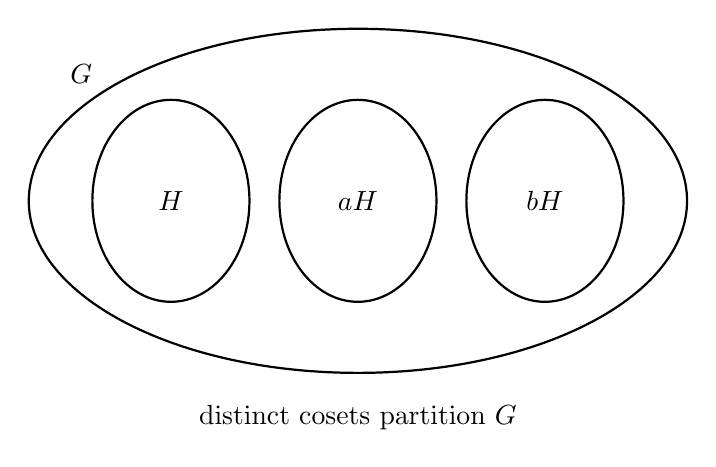
\begin{tikzpicture}[scale=0.95]
\draw[thick] (0,0) ellipse (4.4 and 2.3);
\draw[thick] (-2.5,0) ellipse (1.05 and 1.35);
\draw[thick] (0,0) ellipse (1.05 and 1.35);
\draw[thick] (2.5,0) ellipse (1.05 and 1.35);

\node at (-2.5,0) {\(H\)};
\node at (0,0) {\(aH\)};
\node at (2.5,0) {\(bH\)};
\node at (-3.7,1.7) {\(G\)};
\node at (0,-2.9) {distinct cosets partition \(G\)};
\end{tikzpicture}
\end{center}

%%%%%%%%%%%%%%%%%%%%%%%%%%%%%%%%%%%%%%%%%%%%%%%%%%%%%%%%%%%%
\subsection{Cosets Have Equal Size}
\label{subsec:cosets-equal-size}
%%%%%%%%%%%%%%%%%%%%%%%%%%%%%%%%%%%%%%%%%%%%%%%%%%%%%%%%%%%%

For each \(a\in G\), define

\[ f:H\to aH,\qquad f(h)=ah. \]

This map is bijective.

Therefore,

\[ |aH|=|H| \]

for finite groups.

Every coset has the same number of elements as the subgroup.

%%%%%%%%%%%%%%%%%%%%%%%%%%%%%%%%%%%%%%%%%%%%%%%%%%%%%%%%%%%%
\subsection{Lagrange's Theorem}
\label{subsec:lagrange-theorem}
%%%%%%%%%%%%%%%%%%%%%%%%%%%%%%%%%%%%%%%%%%%%%%%%%%%%%%%%%%%%

\begin{theorem}[Lagrange's Theorem]
If \(G\) is a finite group and \(H\leq G\), then
\[ |G|=[G:H]|H|, \]
where \([G:H]\) is the number of left cosets of \(H\) in \(G\).
\end{theorem}

The notation

\[ [G:H] \]

is read ``the index of \(H\) in \(G\).''

%%%%%%%%%%%%%%%%%%%%%%%%%%%%%%%%%%%%%%%%%%%%%%%%%%%%%%%%%%%%
\subsection{Visual Meaning of Lagrange's Theorem}
\label{subsec:visual-lagrange}
%%%%%%%%%%%%%%%%%%%%%%%%%%%%%%%%%%%%%%%%%%%%%%%%%%%%%%%%%%%%

Suppose a group has \(12\) elements and a subgroup has \(4\) elements.

Then the group must break into

\[ \frac{12}{4}=3 \]

cosets.

\begin{center}
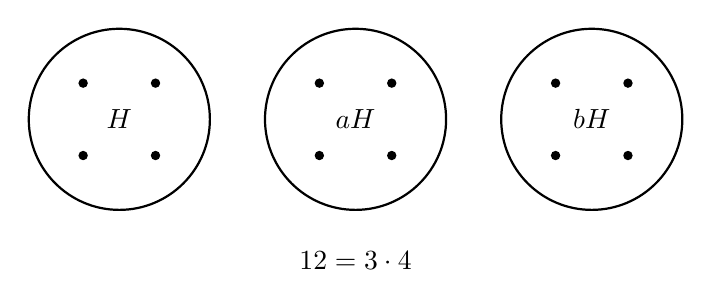
\begin{tikzpicture}
\foreach \x/\lab in {-3/\(H\),0/\(aH\),3/\(bH\)}{
    \draw[thick] (\x,0) circle (1.15);
    \node at (\x,0) {\lab};
    \foreach \ang in {45,135,225,315}{
        \fill ({\x+0.65*cos(\ang)},{0.65*sin(\ang)}) circle (1.7pt);
    }
}
\node at (0,-1.8) {\(12=3\cdot4\)};
\end{tikzpicture}
\end{center}

%%%%%%%%%%%%%%%%%%%%%%%%%%%%%%%%%%%%%%%%%%%%%%%%%%%%%%%%%%%%
\subsection{Proof of Lagrange's Theorem}
\label{subsec:proof-lagrange}
%%%%%%%%%%%%%%%%%%%%%%%%%%%%%%%%%%%%%%%%%%%%%%%%%%%%%%%%%%%%

\begin{proof}
The distinct left cosets of \(H\) partition \(G\).

Each coset contains exactly \(|H|\) elements.

If there are \([G:H]\) distinct cosets, then the total number of elements in
\(G\) is

\[ |G|=[G:H]|H|. \]

Therefore,

\[ |H|\mid|G|. \]
\end{proof}

The symbol

\[ \mid \]

is read ``divides.''

Thus

\[ |H|\mid|G| \]

is read ``the order of \(H\) divides the order of \(G\).''

%%%%%%%%%%%%%%%%%%%%%%%%%%%%%%%%%%%%%%%%%%%%%%%%%%%%%%%%%%%%
\subsection{Consequences of Lagrange's Theorem}
\label{subsec:lagrange-consequences}
%%%%%%%%%%%%%%%%%%%%%%%%%%%%%%%%%%%%%%%%%%%%%%%%%%%%%%%%%%%%

\begin{corollary}
If \(G\) is finite and \(a\in G\), then
\[ |a|\mid|G|. \]
\end{corollary}

This follows because

\[ |\langle a\rangle|=|a|. \]

Another important consequence is

\[ a^{|G|}=e \]

for every \(a\in G\).

%%%%%%%%%%%%%%%%%%%%%%%%%%%%%%%%%%%%%%%%%%%%%%%%%%%%%%%%%%%%
\subsection{Groups of Prime Order}
\label{subsec:groups-prime-order}
%%%%%%%%%%%%%%%%%%%%%%%%%%%%%%%%%%%%%%%%%%%%%%%%%%%%%%%%%%%%

\begin{theorem}
Every group of prime order is cyclic.
\end{theorem}

\begin{proof}
Suppose

\[ |G|=p, \]

where \(p\) is prime.

Choose \(a\neq e\).

By Lagrange's theorem,

\[ |a|\mid p. \]

Since \(a\neq e\),

\[ |a|\neq1. \]

Therefore,

\[ |a|=p. \]

Hence

\[ \langle a\rangle=G. \]
\end{proof}

%%%%%%%%%%%%%%%%%%%%%%%%%%%%%%%%%%%%%%%%%%%%%%%%%%%%%%%%%%%%
\subsection{Normal Subgroups}
\label{subsec:normal-subgroups}
%%%%%%%%%%%%%%%%%%%%%%%%%%%%%%%%%%%%%%%%%%%%%%%%%%%%%%%%%%%%

Left and right cosets need not agree.

A subgroup for which they always agree has special importance.

\begin{definitionbox}{Normal Subgroup}
A subgroup \(N\leq G\) is \emph{normal} if
\[ gN=Ng \]
for every \(g\in G\).
\end{definitionbox}

The notation

\[ N\trianglelefteq G \]

is read ``\(N\) is a normal subgroup of \(G\).''

The symbol

\[ \trianglelefteq \]

is called the normal-subgroup symbol.

%%%%%%%%%%%%%%%%%%%%%%%%%%%%%%%%%%%%%%%%%%%%%%%%%%%%%%%%%%%%
\subsection{Conjugation}
\label{subsec:group-conjugation}
%%%%%%%%%%%%%%%%%%%%%%%%%%%%%%%%%%%%%%%%%%%%%%%%%%%%%%%%%%%%

For \(g,a\in G\), the element

\[ gag^{-1} \]

is called the \emph{conjugate} of \(a\) by \(g\).

A subgroup \(N\leq G\) is normal precisely when

\[ gNg^{-1}=N \]

for every \(g\in G\).

Normality means the subgroup is stable under conjugation by elements of the
larger group.

%%%%%%%%%%%%%%%%%%%%%%%%%%%%%%%%%%%%%%%%%%%%%%%%%%%%%%%%%%%%
\subsection{Normal Subgroups in Abelian Groups}
\label{subsec:normal-abelian}
%%%%%%%%%%%%%%%%%%%%%%%%%%%%%%%%%%%%%%%%%%%%%%%%%%%%%%%%%%%%

\begin{theorem}
Every subgroup of an abelian group is normal.
\end{theorem}

\begin{proof}
Let \(H\leq G\), where \(G\) is abelian.

For every \(g\in G\),

\[ gH=\{gh:h\in H\}. \]

Since \(gh=hg\),

\[ gH=\{hg:h\in H\}=Hg. \]

Therefore,

\[ H\trianglelefteq G. \]
\end{proof}

%%%%%%%%%%%%%%%%%%%%%%%%%%%%%%%%%%%%%%%%%%%%%%%%%%%%%%%%%%%%
\subsection{Quotient Groups}
\label{subsec:quotient-groups}
%%%%%%%%%%%%%%%%%%%%%%%%%%%%%%%%%%%%%%%%%%%%%%%%%%%%%%%%%%%%

Normal subgroups allow the cosets themselves to form a group.

\begin{definitionbox}{Quotient Group}
If \(N\trianglelefteq G\), the \emph{quotient group} is
\[ G/N=\{gN:g\in G\}, \]
with operation
\[ (aN)(bN)=(ab)N. \]
\end{definitionbox}

The notation

\[ G/N \]

is read ``\(G\) modulo \(N\)'' or ``\(G\) quotient \(N\).''

%%%%%%%%%%%%%%%%%%%%%%%%%%%%%%%%%%%%%%%%%%%%%%%%%%%%%%%%%%%%
\subsection{Visualizing a Quotient Group}
\label{subsec:visual-quotient-group}
%%%%%%%%%%%%%%%%%%%%%%%%%%%%%%%%%%%%%%%%%%%%%%%%%%%%%%%%%%%%

A quotient group treats each coset as a single new element.

\begin{center}
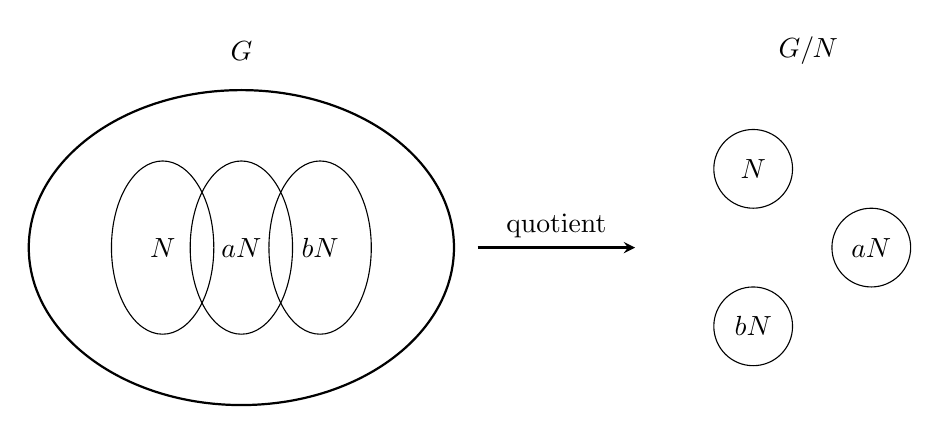
\begin{tikzpicture}[>=stealth]
\draw[thick] (-4,0) ellipse (2.7 and 2);
\draw (-5,0) ellipse (0.65 and 1.1);
\draw (-4,0) ellipse (0.65 and 1.1);
\draw (-3,0) ellipse (0.65 and 1.1);

\node at (-5,0) {\(N\)};
\node at (-4,0) {\(aN\)};
\node at (-3,0) {\(bN\)};
\node at (-4,2.5) {\(G\)};

\draw[->,thick] (-1,0)--(1,0);
\node[above] at (0,0) {quotient};

\node[circle,draw,minimum size=10mm] at (2.5,1) {\(N\)};
\node[circle,draw,minimum size=10mm] at (4,0) {\(aN\)};
\node[circle,draw,minimum size=10mm] at (2.5,-1) {\(bN\)};
\node at (3.2,2.5) {\(G/N\)};
\end{tikzpicture}
\end{center}

The quotient compresses each entire coset into one element of a new group.

%%%%%%%%%%%%%%%%%%%%%%%%%%%%%%%%%%%%%%%%%%%%%%%%%%%%%%%%%%%%
\subsection{Example: Integers Modulo \(n\)}
\label{subsec:quotient-z-nz}
%%%%%%%%%%%%%%%%%%%%%%%%%%%%%%%%%%%%%%%%%%%%%%%%%%%%%%%%%%%%

Because

\[ n\Z\trianglelefteq\Z, \]

we may form

\[ \Z/n\Z. \]

Its elements are

\[ 0+n\Z,\quad1+n\Z,\quad\ldots,\quad(n-1)+n\Z. \]

These correspond to the congruence classes

\[ [0]_n,[1]_n,\ldots,[n-1]_n. \]

Thus modular arithmetic is naturally a quotient-group construction.

%%%%%%%%%%%%%%%%%%%%%%%%%%%%%%%%%%%%%%%%%%%%%%%%%%%%%%%%%%%%
\subsection{Group Homomorphisms}
\label{subsec:group-homomorphisms}
%%%%%%%%%%%%%%%%%%%%%%%%%%%%%%%%%%%%%%%%%%%%%%%%%%%%%%%%%%%%

\begin{definitionbox}{Group Homomorphism}
Let \(G\) and \(H\) be groups. A function
\[ \varphi:G\to H \]
is a \emph{group homomorphism} if
\[ \varphi(ab)=\varphi(a)\varphi(b) \]
for every \(a,b\in G\).
\end{definitionbox}

A homomorphism preserves the group operation.

%%%%%%%%%%%%%%%%%%%%%%%%%%%%%%%%%%%%%%%%%%%%%%%%%%%%%%%%%%%%
\subsection{Homomorphisms Preserve Identity}
\label{subsec:homomorphism-identity}
%%%%%%%%%%%%%%%%%%%%%%%%%%%%%%%%%%%%%%%%%%%%%%%%%%%%%%%%%%%%

\begin{theorem}
If \(\varphi:G\to H\) is a group homomorphism, then
\[ \varphi(e_G)=e_H. \]
\end{theorem}

\begin{proof}
Since

\[ e_Ge_G=e_G, \]

apply \(\varphi\):

\[ \varphi(e_G)\varphi(e_G)=\varphi(e_G). \]

Cancel \(\varphi(e_G)\) to obtain

\[ \varphi(e_G)=e_H. \]
\end{proof}

%%%%%%%%%%%%%%%%%%%%%%%%%%%%%%%%%%%%%%%%%%%%%%%%%%%%%%%%%%%%
\subsection{Homomorphisms Preserve Inverses}
\label{subsec:homomorphism-inverses}
%%%%%%%%%%%%%%%%%%%%%%%%%%%%%%%%%%%%%%%%%%%%%%%%%%%%%%%%%%%%

\begin{theorem}
If \(\varphi:G\to H\) is a homomorphism, then
\[ \varphi(a^{-1})=\varphi(a)^{-1}. \]
\end{theorem}

\begin{proof}
Since

\[ aa^{-1}=e_G, \]

we have

\[ \varphi(a)\varphi(a^{-1})=\varphi(e_G)=e_H. \]

Therefore,

\[ \varphi(a^{-1})=\varphi(a)^{-1}. \]
\end{proof}

%%%%%%%%%%%%%%%%%%%%%%%%%%%%%%%%%%%%%%%%%%%%%%%%%%%%%%%%%%%%
\subsection{Homomorphisms Preserve Powers}
\label{subsec:homomorphism-powers}
%%%%%%%%%%%%%%%%%%%%%%%%%%%%%%%%%%%%%%%%%%%%%%%%%%%%%%%%%%%%

For every integer \(n\),

\[ \varphi(a^n)=\varphi(a)^n. \]

Thus a homomorphism preserves the algebraic behavior generated by repeated
application of the group operation.

%%%%%%%%%%%%%%%%%%%%%%%%%%%%%%%%%%%%%%%%%%%%%%%%%%%%%%%%%%%%
\subsection{Kernel of a Group Homomorphism}
\label{subsec:group-kernel}
%%%%%%%%%%%%%%%%%%%%%%%%%%%%%%%%%%%%%%%%%%%%%%%%%%%%%%%%%%%%

\begin{definitionbox}{Kernel}
For a homomorphism
\[ \varphi:G\to H, \]
the \emph{kernel} is
\[ \Ker(\varphi)=\{g\in G:\varphi(g)=e_H\}. \]
\end{definitionbox}

The kernel records which elements of \(G\) are collapsed to the identity of
\(H\).

%%%%%%%%%%%%%%%%%%%%%%%%%%%%%%%%%%%%%%%%%%%%%%%%%%%%%%%%%%%%
\subsection{Image of a Group Homomorphism}
\label{subsec:group-image}
%%%%%%%%%%%%%%%%%%%%%%%%%%%%%%%%%%%%%%%%%%%%%%%%%%%%%%%%%%%%

\begin{definitionbox}{Image}
For
\[ \varphi:G\to H, \]
the image is
\[ \Image(\varphi)=\{\varphi(g):g\in G\}. \]
\end{definitionbox}

The image is always a subgroup of \(H\).

%%%%%%%%%%%%%%%%%%%%%%%%%%%%%%%%%%%%%%%%%%%%%%%%%%%%%%%%%%%%
\subsection{Kernel and Injectivity}
\label{subsec:kernel-injectivity-group}
%%%%%%%%%%%%%%%%%%%%%%%%%%%%%%%%%%%%%%%%%%%%%%%%%%%%%%%%%%%%

\begin{theorem}
A group homomorphism
\[ \varphi:G\to H \]
is injective if and only if
\[ \Ker(\varphi)=\{e_G\}. \]
\end{theorem}

\begin{proof}
Suppose \(\varphi\) is injective.

If \(g\in\Ker(\varphi)\), then

\[ \varphi(g)=e_H=\varphi(e_G). \]

Injectivity gives

\[ g=e_G. \]

Conversely, suppose

\[ \Ker(\varphi)=\{e_G\}. \]

If

\[ \varphi(a)=\varphi(b), \]

then

\[ \varphi(ab^{-1})=e_H. \]

Thus

\[ ab^{-1}\in\Ker(\varphi). \]

Hence

\[ ab^{-1}=e_G, \]

so

\[ a=b. \]

Therefore \(\varphi\) is injective.
\end{proof}

%%%%%%%%%%%%%%%%%%%%%%%%%%%%%%%%%%%%%%%%%%%%%%%%%%%%%%%%%%%%
\subsection{Kernels Are Normal}
\label{subsec:kernels-normal}
%%%%%%%%%%%%%%%%%%%%%%%%%%%%%%%%%%%%%%%%%%%%%%%%%%%%%%%%%%%%

\begin{theorem}
If
\[ \varphi:G\to H \]
is a group homomorphism, then
\[ \Ker(\varphi)\trianglelefteq G. \]
\end{theorem}

This theorem explains one of the central reasons normal subgroups matter:
they arise naturally as kernels of homomorphisms.

%%%%%%%%%%%%%%%%%%%%%%%%%%%%%%%%%%%%%%%%%%%%%%%%%%%%%%%%%%%%
\subsection{Isomorphisms}
\label{subsec:group-isomorphisms}
%%%%%%%%%%%%%%%%%%%%%%%%%%%%%%%%%%%%%%%%%%%%%%%%%%%%%%%%%%%%

A bijective group homomorphism is a group isomorphism.

If such a map exists, we write

\[ G\cong H. \]

Isomorphic groups may have completely different elements while possessing the
same group structure.

%%%%%%%%%%%%%%%%%%%%%%%%%%%%%%%%%%%%%%%%%%%%%%%%%%%%%%%%%%%%
\subsection{A Commutative Diagram}
\label{subsec:group-commutative-diagram}
%%%%%%%%%%%%%%%%%%%%%%%%%%%%%%%%%%%%%%%%%%%%%%%%%%%%%%%%%%%%

Structure preservation can be displayed with a commutative diagram.

\[
\begin{tikzcd}
G\times G \arrow[r,"*"] \arrow[d,"\varphi\times\varphi"'] &
G \arrow[d,"\varphi"]\\
H\times H \arrow[r,"\circ"] &
H
\end{tikzcd}
\]

The diagram is said to \emph{commute} because either path gives the same
result.

Starting with \((a,b)\),

\[ \varphi(a*b)=\varphi(a)\circ\varphi(b). \]

%%%%%%%%%%%%%%%%%%%%%%%%%%%%%%%%%%%%%%%%%%%%%%%%%%%%%%%%%%%%
\subsection{First Isomorphism Theorem}
\label{subsec:first-isomorphism-theorem-groups}
%%%%%%%%%%%%%%%%%%%%%%%%%%%%%%%%%%%%%%%%%%%%%%%%%%%%%%%%%%%%

\begin{theorem}[First Isomorphism Theorem for Groups]
Let
\[ \varphi:G\to H \]
be a group homomorphism. Then
\[ G/\Ker(\varphi)\cong\Image(\varphi). \]
\end{theorem}

This is one of the central structural results in group theory.

It says that once the elements collapsed by \(\varphi\) are identified, what
remains is structurally identical to the image.

%%%%%%%%%%%%%%%%%%%%%%%%%%%%%%%%%%%%%%%%%%%%%%%%%%%%%%%%%%%%
\subsection{Visualizing the First Isomorphism Theorem}
\label{subsec:visual-first-isomorphism}
%%%%%%%%%%%%%%%%%%%%%%%%%%%%%%%%%%%%%%%%%%%%%%%%%%%%%%%%%%%%

\begin{center}
\begin{tikzpicture}[
    node distance=16mm,
    box/.style={draw,rounded corners,align=center,inner sep=5pt},
    >=stealth
]
\node[box] (G) {\(G\)};
\node[box,right=of G] (Q) {\(G/\Ker(\varphi)\)};
\node[box,right=of Q] (I) {\(\Image(\varphi)\)};

\draw[->,thick] (G)--node[above]{collapse kernel}(Q);
\draw[->,thick] (Q)--node[above]{isomorphism}(I);
\end{tikzpicture}
\end{center}

The kernel measures exactly the information lost by the homomorphism.

%%%%%%%%%%%%%%%%%%%%%%%%%%%%%%%%%%%%%%%%%%%%%%%%%%%%%%%%%%%%
\subsection{Worked Example: A Homomorphism and Its Kernel}
\label{subsec:worked-group-homomorphism}
%%%%%%%%%%%%%%%%%%%%%%%%%%%%%%%%%%%%%%%%%%%%%%%%%%%%%%%%%%%%

\begin{workedexamplebox}{Reduction Modulo \(4\)}

Define

\[ \varphi:\Z\to\Z_4,\qquad \varphi(k)=[k]_4. \]

Determine the kernel and image.

\begin{tabularx}{\textwidth}{@{}>{\raggedright\arraybackslash}p{0.42\textwidth}X@{}}
Find elements mapped to the identity. & \(\varphi(k)=[0]_4\)\\
Interpret the condition. & \(k\equiv0\pmod4\)\\
Write the kernel. & \(\Ker(\varphi)=4\Z\)\\
Determine reachable classes. & \([0]_4,[1]_4,[2]_4,[3]_4\)
\end{tabularx}

Therefore,

\[ \Image(\varphi)=\Z_4. \]

\begin{answerbox}
\[ \Ker(\varphi)=4\Z,\qquad\Image(\varphi)=\Z_4. \]
\end{answerbox}
\end{workedexamplebox}

The First Isomorphism Theorem gives

\[ \Z/4\Z\cong\Z_4. \]

%%%%%%%%%%%%%%%%%%%%%%%%%%%%%%%%%%%%%%%%%%%%%%%%%%%%%%%%%%%%
\subsection{Direct Products}
\label{subsec:direct-products-groups}
%%%%%%%%%%%%%%%%%%%%%%%%%%%%%%%%%%%%%%%%%%%%%%%%%%%%%%%%%%%%

Groups can be combined to create larger groups.

\begin{definitionbox}{Direct Product}
If \(G\) and \(H\) are groups, their \emph{direct product} is
\[ G\times H=\{(g,h):g\in G,\ h\in H\}, \]
with componentwise operation
\[ (g_1,h_1)(g_2,h_2)=(g_1g_2,h_1h_2). \]
\end{definitionbox}

The identity is

\[ (e_G,e_H), \]

and

\[ (g,h)^{-1}=(g^{-1},h^{-1}). \]

%%%%%%%%%%%%%%%%%%%%%%%%%%%%%%%%%%%%%%%%%%%%%%%%%%%%%%%%%%%%
\subsection{Example of a Direct Product}
\label{subsec:direct-product-example}
%%%%%%%%%%%%%%%%%%%%%%%%%%%%%%%%%%%%%%%%%%%%%%%%%%%%%%%%%%%%

Consider

\[ \Z_2\times\Z_3. \]

Its elements are

\[ (0,0),(0,1),(0,2),(1,0),(1,1),(1,2). \]

Therefore,

\[ |\Z_2\times\Z_3|=6. \]

In fact,

\[ \Z_2\times\Z_3\cong\Z_6. \]

This is closely related to the Chinese Remainder Theorem.

%%%%%%%%%%%%%%%%%%%%%%%%%%%%%%%%%%%%%%%%%%%%%%%%%%%%%%%%%%%%
\subsection{Group Actions}
\label{subsec:group-actions}
%%%%%%%%%%%%%%%%%%%%%%%%%%%%%%%%%%%%%%%%%%%%%%%%%%%%%%%%%%%%

Groups frequently describe transformations acting on other mathematical
objects.

\begin{definitionbox}{Group Action}
A \emph{group action} of \(G\) on a set \(X\) assigns to every \(g\in G\) and
\(x\in X\) an element
\[ g\cdot x\in X \]
such that
\[ e\cdot x=x \]
and
\[ (gh)\cdot x=g\cdot(h\cdot x). \]
\end{definitionbox}

The dot in

\[ g\cdot x \]

denotes the action and is read ``\(g\) acts on \(x\).''

%%%%%%%%%%%%%%%%%%%%%%%%%%%%%%%%%%%%%%%%%%%%%%%%%%%%%%%%%%%%
\subsection{Visualizing a Group Action}
\label{subsec:visual-group-action}
%%%%%%%%%%%%%%%%%%%%%%%%%%%%%%%%%%%%%%%%%%%%%%%%%%%%%%%%%%%%

\begin{center}
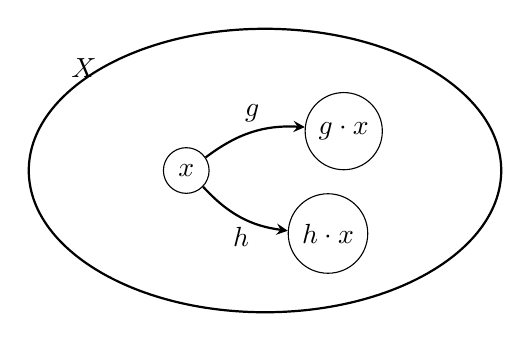
\begin{tikzpicture}[>=stealth]
\draw[thick] (0,0) ellipse (3 and 1.8);
\node at (-2.3,1.3) {\(X\)};

\node[circle,draw] (x) at (-1,0) {\(x\)};
\node[circle,draw] (gx) at (1,0.5) {\(g\cdot x\)};
\node[circle,draw] (hx) at (0.8,-0.8) {\(h\cdot x\)};

\draw[->,thick] (x) to[bend left=20] node[above]{\(g\)} (gx);
\draw[->,thick] (x) to[bend right=20] node[below]{\(h\)} (hx);
\end{tikzpicture}
\end{center}

Group actions connect abstract group elements to concrete transformations.

%%%%%%%%%%%%%%%%%%%%%%%%%%%%%%%%%%%%%%%%%%%%%%%%%%%%%%%%%%%%
\subsection{Orbits}
\label{subsec:orbits}
%%%%%%%%%%%%%%%%%%%%%%%%%%%%%%%%%%%%%%%%%%%%%%%%%%%%%%%%%%%%

\begin{definitionbox}{Orbit}
If \(G\) acts on \(X\), the \emph{orbit} of \(x\in X\) is
\[ \operatorname{Orb}(x)=\{g\cdot x:g\in G\}. \]
\end{definitionbox}

The orbit consists of every point reachable from \(x\) through the group
action.

%%%%%%%%%%%%%%%%%%%%%%%%%%%%%%%%%%%%%%%%%%%%%%%%%%%%%%%%%%%%
\subsection{Stabilizers}
\label{subsec:stabilizers}
%%%%%%%%%%%%%%%%%%%%%%%%%%%%%%%%%%%%%%%%%%%%%%%%%%%%%%%%%%%%

\begin{definitionbox}{Stabilizer}
The \emph{stabilizer} of \(x\in X\) is
\[ \operatorname{Stab}(x)=\{g\in G:g\cdot x=x\}. \]
\end{definitionbox}

The stabilizer consists of group elements that leave \(x\) fixed.

It is a subgroup of \(G\).

%%%%%%%%%%%%%%%%%%%%%%%%%%%%%%%%%%%%%%%%%%%%%%%%%%%%%%%%%%%%
\subsection{Orbit--Stabilizer Theorem}
\label{subsec:orbit-stabilizer}
%%%%%%%%%%%%%%%%%%%%%%%%%%%%%%%%%%%%%%%%%%%%%%%%%%%%%%%%%%%%

\begin{theorem}[Orbit--Stabilizer Theorem]
If a finite group \(G\) acts on \(X\), then for \(x\in X\),
\[ |G|=|\operatorname{Orb}(x)|\,|\operatorname{Stab}(x)|. \]
\end{theorem}

Equivalently,

\[ |\operatorname{Orb}(x)|=[G:\operatorname{Stab}(x)]. \]

This is an important bridge between group structure and symmetry counting.

%%%%%%%%%%%%%%%%%%%%%%%%%%%%%%%%%%%%%%%%%%%%%%%%%%%%%%%%%%%%
\subsection{Worked Example: Square Vertex Orbit}
\label{subsec:worked-square-orbit}
%%%%%%%%%%%%%%%%%%%%%%%%%%%%%%%%%%%%%%%%%%%%%%%%%%%%%%%%%%%%

\begin{workedexamplebox}{Orbit and Stabilizer of a Square Vertex}

Let \(D_4\) act on the four vertices of a square.

Choose one vertex \(v\).

\begin{tabularx}{\textwidth}{@{}>{\raggedright\arraybackslash}p{0.42\textwidth}X@{}}
Count all square symmetries. & \(|D_4|=8\)\\
Determine the orbit of \(v\). & \(|\operatorname{Orb}(v)|=4\)\\
Apply orbit--stabilizer. & \(8=4|\operatorname{Stab}(v)|\)\\
Solve. & \(|\operatorname{Stab}(v)|=2\)
\end{tabularx}

\begin{answerbox}
Exactly \(2\) symmetries of the square fix a chosen vertex.
\end{answerbox}
\end{workedexamplebox}

%%%%%%%%%%%%%%%%%%%%%%%%%%%%%%%%%%%%%%%%%%%%%%%%%%%%%%%%%%%%
\subsection{Cayley's Theorem}
\label{subsec:cayleys-theorem}
%%%%%%%%%%%%%%%%%%%%%%%%%%%%%%%%%%%%%%%%%%%%%%%%%%%%%%%%%%%%

Groups were motivated partly by permutations, but the connection is much
deeper.

\begin{theorem}[Cayley's Theorem]
Every group is isomorphic to a subgroup of a symmetric group.
\end{theorem}

For each \(g\in G\), define the left translation

\[ L_g:G\to G,\qquad L_g(x)=gx. \]

Each \(L_g\) is a permutation of \(G\).

The map

\[ g\mapsto L_g \]

embeds \(G\) into the group of permutations of its underlying set.

Thus every abstract group can be realized concretely as a group of
permutations.

%%%%%%%%%%%%%%%%%%%%%%%%%%%%%%%%%%%%%%%%%%%%%%%%%%%%%%%%%%%%
\subsection{Structural Map of Basic Group Theory}
\label{subsec:group-theory-structure-map}
%%%%%%%%%%%%%%%%%%%%%%%%%%%%%%%%%%%%%%%%%%%%%%%%%%%%%%%%%%%%

\begin{center}
\begin{tikzpicture}[
    node distance=11mm and 15mm,
    box/.style={draw,rounded corners,align=center,inner sep=4pt,font=\small},
    >=stealth
]
\node[box] (group) {Group};
\node[box,below left=of group] (sub) {Subgroups};
\node[box,below right=of group] (hom) {Homomorphisms};
\node[box,below=of sub] (coset) {Cosets};
\node[box,below=of hom] (kernel) {Kernels};
\node[box,below=of coset] (normal) {Normal\\subgroups};
\node[box,below=of kernel] (image) {Images};
\node[box,below right=of normal] (quotient) {Quotient groups};
\node[box,below=of quotient] (iso) {Isomorphism\\theorems};

\draw[->] (group)--(sub);
\draw[->] (group)--(hom);
\draw[->] (sub)--(coset);
\draw[->] (hom)--(kernel);
\draw[->] (hom)--(image);
\draw[->] (coset)--(normal);
\draw[->] (kernel)--(normal);
\draw[->] (normal)--(quotient);
\draw[->] (image)--(quotient);
\draw[->] (quotient)--(iso);
\end{tikzpicture}
\end{center}

This diagram summarizes one of the major conceptual pathways through elementary
group theory.

%%%%%%%%%%%%%%%%%%%%%%%%%%%%%%%%%%%%%%%%%%%%%%%%%%%%%%%%%%%%
\subsection{Common Errors in Group Theory}
\label{subsec:common-group-errors}
%%%%%%%%%%%%%%%%%%%%%%%%%%%%%%%%%%%%%%%%%%%%%%%%%%%%%%%%%%%%

\subsubsection{Assuming Every Group Is Abelian}

The equation

\[ ab=ba \]

cannot be used unless commutativity has been established.

%%%%%%%%%%%%%%%%%%%%%%%%%%%%%%%%%%%%%%%%%%%%%%%%%%%%%%%%%%%%
\subsubsection{Cancelling in the Wrong Order}

From

\[ ax=b, \]

the correct solution is

\[ x=a^{-1}b. \]

It is generally incorrect to write

\[ x=ba^{-1}. \]

%%%%%%%%%%%%%%%%%%%%%%%%%%%%%%%%%%%%%%%%%%%%%%%%%%%%%%%%%%%%
\subsubsection{Forgetting to Reverse Products When Inverting}

The correct rule is

\[ (ab)^{-1}=b^{-1}a^{-1}. \]

%%%%%%%%%%%%%%%%%%%%%%%%%%%%%%%%%%%%%%%%%%%%%%%%%%%%%%%%%%%%
\subsubsection{Confusing Group Order and Element Order}

The expressions

\[ |G| \]

and

\[ |a| \]

refer to different concepts.

The first is the number of elements in a finite group.

The second is the smallest positive exponent returning \(a\) to the identity.

%%%%%%%%%%%%%%%%%%%%%%%%%%%%%%%%%%%%%%%%%%%%%%%%%%%%%%%%%%%%
\subsubsection{Assuming Every Subgroup Is Normal}

Every subgroup of an abelian group is normal, but this is false for general
groups.

%%%%%%%%%%%%%%%%%%%%%%%%%%%%%%%%%%%%%%%%%%%%%%%%%%%%%%%%%%%%
\subsubsection{Assuming the Converse of Lagrange's Theorem}

Lagrange's theorem says

\[ H\leq G\Longrightarrow |H|\mid|G|. \]

It does not say that every divisor of \(|G|\) must correspond to a subgroup
of that order.

%%%%%%%%%%%%%%%%%%%%%%%%%%%%%%%%%%%%%%%%%%%%%%%%%%%%%%%%%%%%
\subsubsection{Confusing Cosets with Subgroups}

A coset

\[ aH \]

need not itself be a subgroup.

If \(a\notin H\), then the identity of \(G\) is generally not contained in
\(aH\).

%%%%%%%%%%%%%%%%%%%%%%%%%%%%%%%%%%%%%%%%%%%%%%%%%%%%%%%%%%%%
\subsubsection{Ignoring the Operation}

A group is not determined by its set alone.

The structures

\[ (\Z,+) \]

and

\[ (\Z,\cdot) \]

have the same underlying set but very different algebraic behavior.

%%%%%%%%%%%%%%%%%%%%%%%%%%%%%%%%%%%%%%%%%%%%%%%%%%%%%%%%%%%%
\subsection{Applications of Group Theory}
\label{subsec:group-theory-applications}
%%%%%%%%%%%%%%%%%%%%%%%%%%%%%%%%%%%%%%%%%%%%%%%%%%%%%%%%%%%%

Group theory appears throughout mathematics and science.

\begin{applicationbox}
\textbf{Geometry.}
Symmetry groups classify rotations, reflections, and other transformations
that preserve geometric objects.

\medskip

\textbf{Number Theory.}
Groups arise naturally in modular arithmetic and the study of units modulo
\(n\).

\medskip

\textbf{Linear Algebra.}
Invertible matrices form general linear groups, while determinant conditions
produce important matrix subgroups.

\medskip

\textbf{Field and Galois Theory.}
Groups encode symmetries among roots of polynomial equations.

\medskip

\textbf{Topology.}
The fundamental group records information about loops in topological spaces.

\medskip

\textbf{Physics.}
Symmetry groups describe conservation laws, particle symmetries, rotations,
and transformations of physical systems.

\medskip

\textbf{Chemistry.}
Molecular symmetry can be studied using finite groups.

\medskip

\textbf{Cryptography.}
Many cryptographic systems rely on computational problems in finite groups.
\end{applicationbox}

%%%%%%%%%%%%%%%%%%%%%%%%%%%%%%%%%%%%%%%%%%%%%%%%%%%%%%%%%%%%
\subsection{Exercises}
\label{subsec:group-theory-exercises}
%%%%%%%%%%%%%%%%%%%%%%%%%%%%%%%%%%%%%%%%%%%%%%%%%%%%%%%%%%%%

\begin{exercise}[1]
Verify that \((\Z,+)\) satisfies the group axioms.
\end{exercise}

\begin{exercise}[1]
Explain why \((\N,+)\) is not a group.
\end{exercise}

\begin{exercise}[1]
Explain why \((\Z,\cdot)\) is not a group.
\end{exercise}

\begin{exercise}[1]
Show that \((\Q\setminus\{0\},\cdot)\) is an abelian group.
\end{exercise}

\begin{exercise}[1]
Find the identity and inverse of each element in \(\Z_5\) under addition.
\end{exercise}

\begin{exercise}[2]
Prove that the identity element of a group is unique.
\end{exercise}

\begin{exercise}[2]
Prove that every element of a group has a unique inverse.
\end{exercise}

\begin{exercise}[2]
Prove the right cancellation law.
\end{exercise}

\begin{exercise}[2]
Prove
\[ (abc)^{-1}=c^{-1}b^{-1}a^{-1}. \]
\end{exercise}

\begin{exercise}[2]
Solve
\[ axb=c \]
for \(x\) in an arbitrary group.
\end{exercise}

\begin{exercise}[1]
Determine the order of every element of \(\Z_6\).
\end{exercise}

\begin{exercise}[2]
Find every generator of \(\Z_8\).
\end{exercise}

\begin{exercise}[2]
Find every generator of \(\Z_{10}\).
\end{exercise}

\begin{exercise}[2]
Prove that every cyclic group is abelian.
\end{exercise}

\begin{exercise}[2]
Give an example showing that the converse is false.
\end{exercise}

\begin{exercise}[2]
Use the subgroup test to prove
\[ 5\Z\leq\Z. \]
\end{exercise}

\begin{exercise}[2]
Determine whether the odd integers form a subgroup of \((\Z,+)\).
\end{exercise}

\begin{exercise}[2]
Prove that the intersection of two subgroups is a subgroup.
\end{exercise}

\begin{exercise}[2]
Give an example showing that the union of two subgroups need not be a
subgroup.
\end{exercise}

\begin{exercise}[1]
Write the permutation
\[
\begin{pmatrix}
1&2&3&4&5\\
3&5&1&2&4
\end{pmatrix}
\]
in cycle notation.
\end{exercise}

\begin{exercise}[2]
Write
\[ (1\,4\,3)(2\,5) \]
in two-line notation.
\end{exercise}

\begin{exercise}[2]
Express
\[ (1\,2\,3\,4) \]
as a product of transpositions.
\end{exercise}

\begin{exercise}[2]
Determine whether the permutation
\[ (1\,2\,3)(4\,5) \]
is even or odd.
\end{exercise}

\begin{exercise}[1]
How many elements are in \(S_5\)?
\end{exercise}

\begin{exercise}[1]
How many elements are in \(A_5\)?
\end{exercise}

\begin{exercise}[2]
List the rotational symmetries of a square.
\end{exercise}

\begin{exercise}[2]
Explain why the symmetry group of a square is nonabelian.
\end{exercise}

\begin{exercise}[2]
List the cosets of \(4\Z\) in \(\Z\).
\end{exercise}

\begin{exercise}[2]
Find
\[ [\Z:5\Z]. \]
\end{exercise}

\begin{exercise}[2]
Suppose \(|G|=24\). List all possible subgroup orders allowed by Lagrange's
theorem.
\end{exercise}

\begin{exercise}[2]
Suppose \(|G|=15\). What are the possible orders of an element of \(G\)?
\end{exercise}

\begin{exercise}[2]
Prove that a group of order \(7\) is cyclic.
\end{exercise}

\begin{exercise}[3]
Prove that any group of prime order is cyclic.
\end{exercise}

\begin{exercise}[2]
Prove that every subgroup of an abelian group is normal.
\end{exercise}

\begin{exercise}[2]
Show that
\[ n\Z\trianglelefteq\Z. \]
\end{exercise}

\begin{exercise}[2]
Describe the quotient group
\[ \Z/3\Z. \]
\end{exercise}

\begin{exercise}[2]
Let
\[ \varphi:\Z\to\Z_6,\qquad\varphi(n)=[n]_6. \]
Find the kernel and image.
\end{exercise}

\begin{exercise}[3]
Use the First Isomorphism Theorem to show
\[ \Z/6\Z\cong\Z_6. \]
\end{exercise}

\begin{exercise}[2]
Prove that the image of a group homomorphism is a subgroup.
\end{exercise}

\begin{exercise}[3]
Prove that the kernel of a group homomorphism is normal.
\end{exercise}

\begin{exercise}[2]
Determine whether
\[ \varphi:\Z\to\Z,\qquad\varphi(n)=3n \]
is a group homomorphism under addition. Determine whether it is injective or
surjective.
\end{exercise}

\begin{exercise}[2]
List the elements of
\[ \Z_2\times\Z_4. \]
Determine its order.
\end{exercise}

\begin{exercise}[3]
Determine whether
\[ \Z_2\times\Z_2 \]
is isomorphic to \(\Z_4\). Justify your answer using element orders.
\end{exercise}

\begin{exercise}[2]
Let \(D_4\) act on the vertices of a square. Determine the orbit of one vertex.
\end{exercise}

\begin{exercise}[2]
For the same action, determine the stabilizer of one vertex.
\end{exercise}

\begin{exercise}[3]
Verify the Orbit--Stabilizer Theorem for the action of \(D_4\) on the vertices
of a square.
\end{exercise}

\begin{exercise}[3]
Explain in your own words why Cayley's theorem allows permutation groups to be
viewed as universal models for groups.
\end{exercise}

%%%%%%%%%%%%%%%%%%%%%%%%%%%%%%%%%%%%%%%%%%%%%%%%%%%%%%%%%%%%
\subsection{Section Connections}
\label{subsec:group-theory-connections}
%%%%%%%%%%%%%%%%%%%%%%%%%%%%%%%%%%%%%%%%%%%%%%%%%%%%%%%%%%%%

\chapterconnection{
Group theory provides the canonical theory of algebraic symmetry and
invertibility. The next sections extend these structural ideas in several
directions. Ring theory introduces a second compatible operation. Field theory
adds sufficiently strong multiplicative inverses to support division and
linear algebra. Galois theory connects groups to field extensions and
polynomial equations. Module theory generalizes vector spaces by replacing
field scalars with ring scalars. Representation theory later studies groups
through homomorphisms into groups of invertible linear transformations.
Groups also reappear in geometry, topology, number theory, differential
equations, combinatorics, and mathematical physics.
}

%%%%%%%%%%%%%%%%%%%%%%%%%%%%%%%%%%%%%%%%%%%%%%%%%%%%%%%%%%%%
% SECTION SOURCE TRACKING
%%%%%%%%%%%%%%%%%%%%%%%%%%%%%%%%%%%%%%%%%%%%%%%%%%%%%%%%%%%%

%------------------------------------------------------------
% 1.4 Group Theory
%------------------------------------------------------------
%
% Sources:
%   - Thomas W. Judson, Abstract Algebra: Theory and Applications.
%     Key: judson2025abstractalgebra
%
% Used for:
%   - group axioms and elementary consequences;
%   - cyclic groups and subgroup structure;
%   - permutation and symmetry groups;
%   - cosets and Lagrange's theorem;
%   - normal subgroups and quotient groups;
%   - group homomorphisms, kernels, and images;
%   - isomorphism concepts;
%   - direct products;
%   - introductory group actions;
%   - standard proof patterns and examples.
%
% Notes:
%   - Group theory is treated here as the canonical location for group
%     structure, so later sections should reference these results rather
%     than redeveloping them.
%   - Advanced group classification, Sylow theory, solvable groups, free
%     groups, presentations, and related deeper topics may be expanded
%     later if a dedicated advanced group theory subdivision is added.
%   - Visualizations and exposition are independently developed for this text.
%
\nocite{judson2025abstractalgebra}